\documentclass{scrartcl}
\usepackage[utf8]{inputenc}
\usepackage[english]{babel} % Trennung nach der neuen deutschen Rechtschreibung
\usepackage[utf8]{inputenc}
\usepackage[T1]{fontenc}
\usepackage{lmodern}
\usepackage{subcaption}
\usepackage{chemformula}
\usepackage{placeins}
\usepackage{multirow}

\usepackage[backend=biber, sorting=ynt]{biblatex} %Imports biblatex package
\addbibresource{citation.bib} %Import the bibliography file

\usepackage{amsmath} % Erweiterte Mathematik-Umgebung
\usepackage{amsfonts} % zusätzliche Mathematik-Schrifttypen (v.a. \mathbb für Mengen)
\usepackage{ulem}

\usepackage{graphics}%soll beim Graphiken einfügen hilfreich sein
\usepackage{graphicx}
\usepackage{wrapfig}%lässt Textumflossene Bildeinbindung zu
\usepackage{epstopdf}%soll eps in pdf umwandeln

\usepackage{amsthm}

\usepackage[a4paper, portrait, margin=2.5cm]{geometry}

\titlehead{\centering University of Luxemburg}
\subject{Travaux Pratiques}
\title{Quantization}
\date{TP Session 10/03/2021}
\author{Florence Schmerber (0201845640),
Louis-Hendrik Barboutie(020157041C)}
\begin{document}

\maketitle

\clearpage

\tableofcontents

\listoffigures
	
\clearpage

\section{Introduction}
The aim of today's experiment is to re-do the same experiments conducted in the 20th century, that quantized atomic energies and the energy of light, which are the Franck-Hertz experiment and the photoelectric effect. In the first part of this TP, we will focus on the Frank-Hertz experiment using neon and mercury and then on the photoelectric effect. Using Bohr's second postulate, atoms can absorb energy in quantized steps and thus can be excited. The goal is to analyse the current inside the tube filled with gas when we increase the voltage. 
\newline 
The photoelectric effect describes the emission of electrons from an illuminated metal. These photo electrons are independent of the intensity of the light, in fact only its frequency is significant. Einstein explained that the particles that constitute light, photons, have an energy of $E = h \cdot \nu$. The necessary energy to remove an electron from the surface of the metal is called work function $\Phi_{cathode}$ and the voltage where no current can be detected is called stopping potential $V_0$. In order to determine Planck's constant, we will be measuring the stopping potential and then analysing the photo diode.

\section{Franck-Hertz}

\subsection{Setup}

\begin{wrapfigure}{l}{0.3 \textwidth}
\centering
    \includegraphics[width=0.3\textwidth]{Franck_2.jpg}
    \caption{Franck-Hertz experiment tube}
\end{wrapfigure}

This experiment necessitates following equipment:

\begin{itemize}
    \item A mercury gas lamp
    \item A neon gas lamp
    \item a computer with data handling software
\end{itemize}

\noindent The vacuum tube is filled with a gas of our choice. When current passes through the cathode, it undergoes thermionic emission, i.e. it will emit electrons. These are drawn to the positively charged grid (denoted with G) and get accelerated throughout the potential difference. On the other side of the grid, a counter voltage is applied, so that only electrons with enough kinetic energy can reach the anode. Between the anode and cathode are atoms of our gas, with which the electrons can collide \cite{Franck}. The intensity of arriving electrons is measured by the resulting current. An additional modifiable parameter is the temperature of the tube, which allows to study the influence of heating the tube.

\subsection{Method}
The goal here is to determine the excitation energy of both mercury and neon. The excitation energy is the necessary energy to excite the gas through a inelastic collision with the accelerated electron. When this collision happens, the current drops sharply. This is due to the loss of energy of the accelerated electron, that now don't have enough energy to reach the anode. The energy is then released in the form of light by the gas. If the electrons don't have the energy required to excite the gas, elastic collisions are occurring which have little effect on the initial energy of the electron (see appendix).
So in order to determine the excitation energy, we will simply read the current as a function of applied voltage. As a result, we get a graph with peaks that are equally distant to each other.
At room temperature, Mercury is in liquid state, so we can't do collisions between electrons and single atoms. We need to heat the mercury tube, so that it is in gaseous state and fills the space between the anode and cathode.

\subsection{Results}

\subsubsection{Mercury}
\begin{figure}[h]
\begin{center}
\begin{subfigure}{0.49 \textwidth}
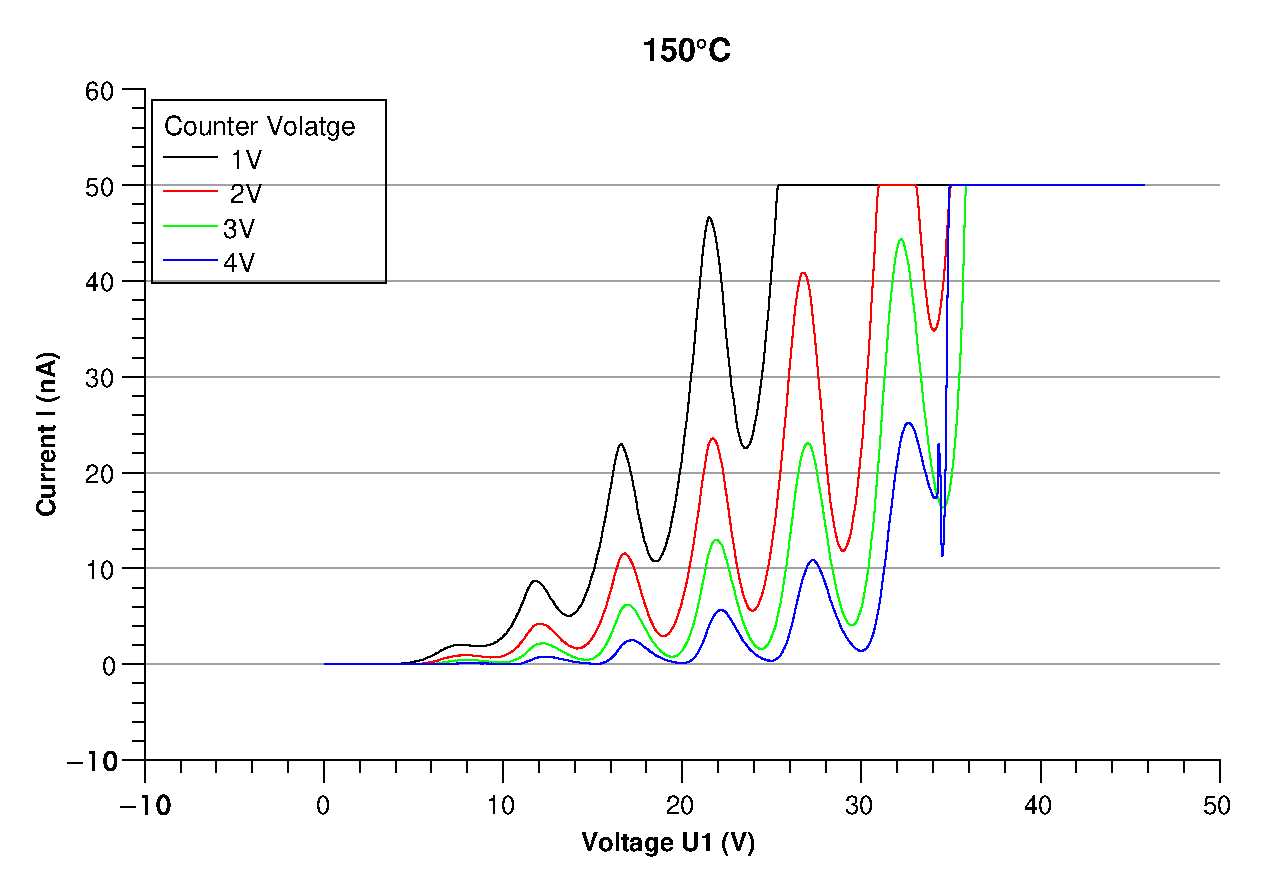
\includegraphics[width=8cm]{150.eps}
\caption{I(V) for 150°C}
\end{subfigure}
\begin{subfigure}{0.49 \textwidth}
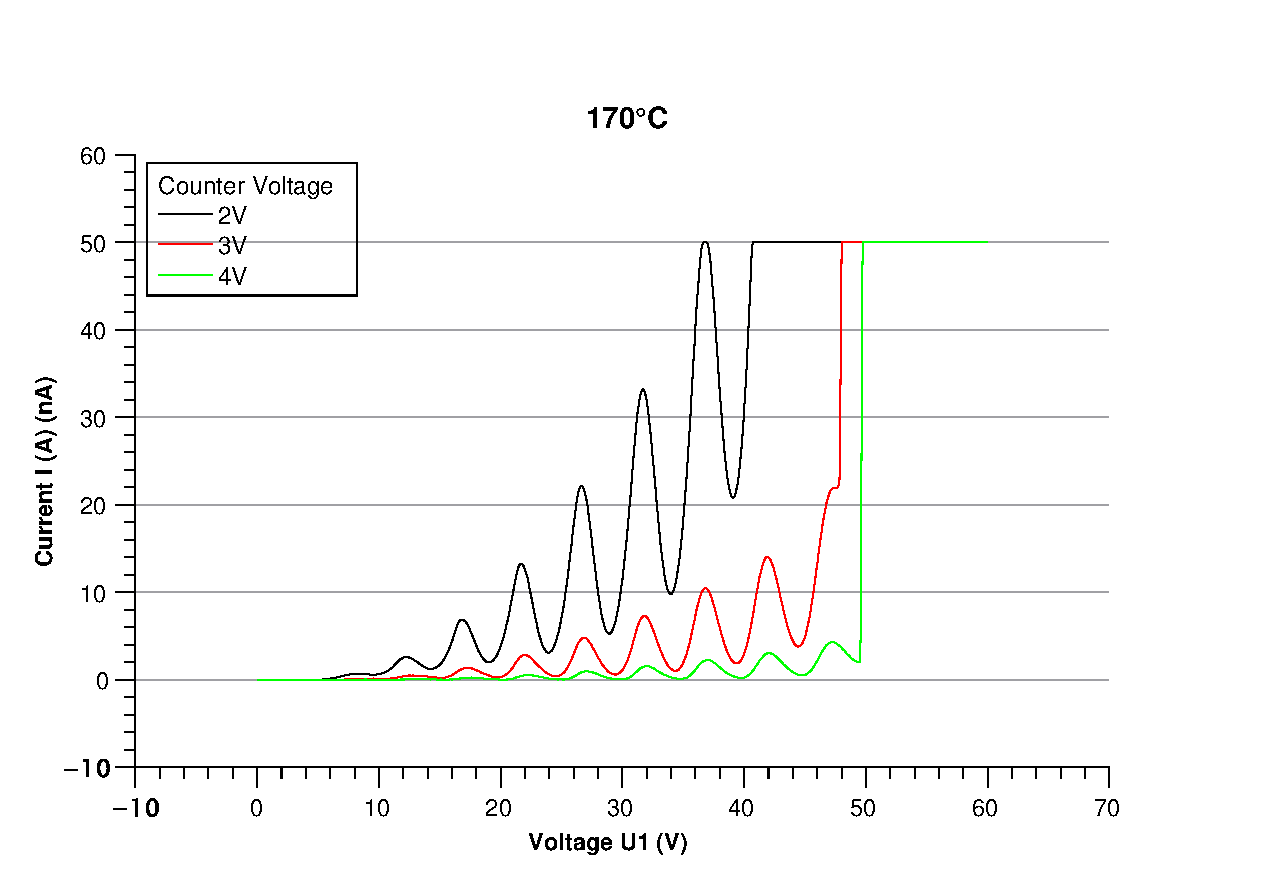
\includegraphics[width=8cm]{170.eps}
\caption{I(V) for 170°C}
\end{subfigure}
\begin{subfigure}{0.49 \textwidth}
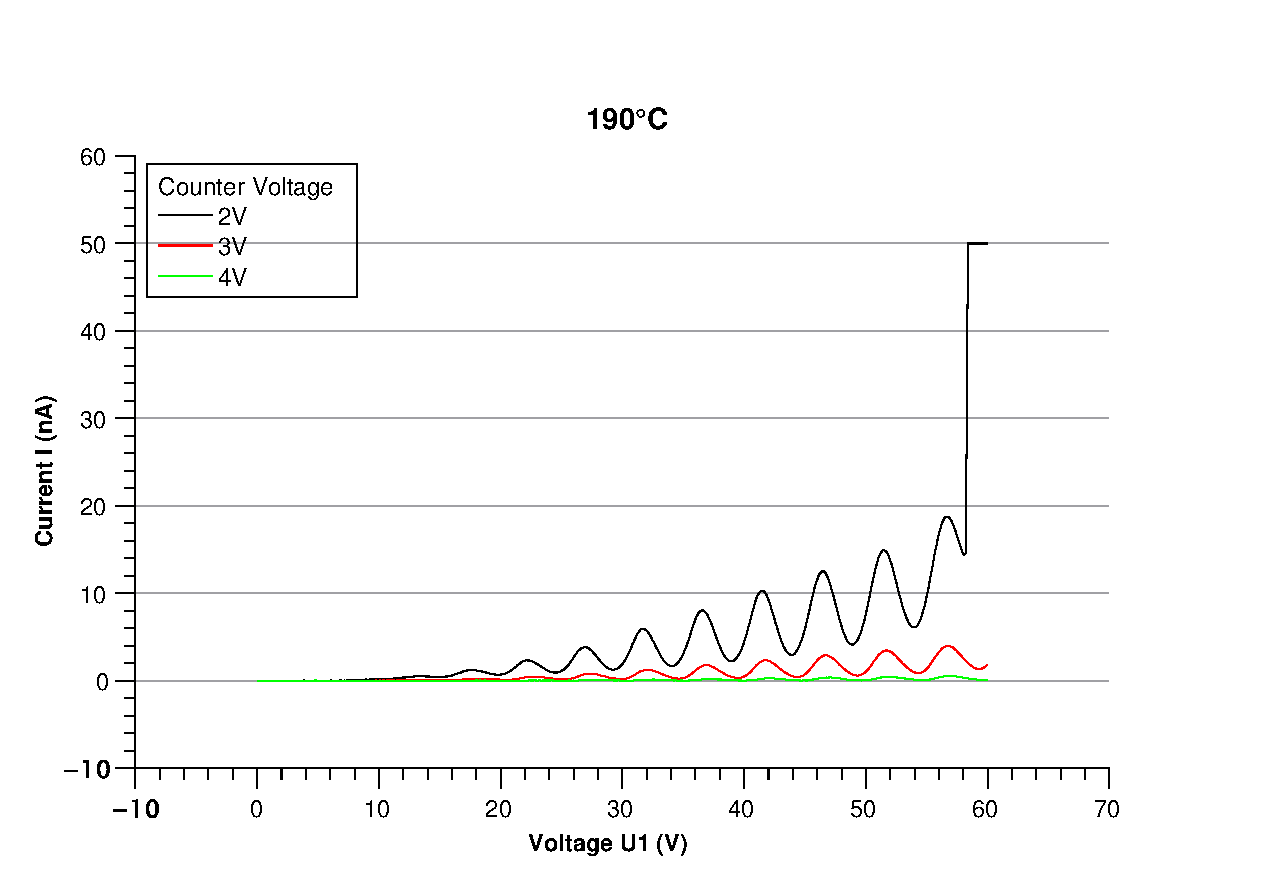
\includegraphics[width=8cm]{190.eps}
\caption{I(V) for 190°C}
\end{subfigure}
\begin{subfigure}{0.49 \textwidth}
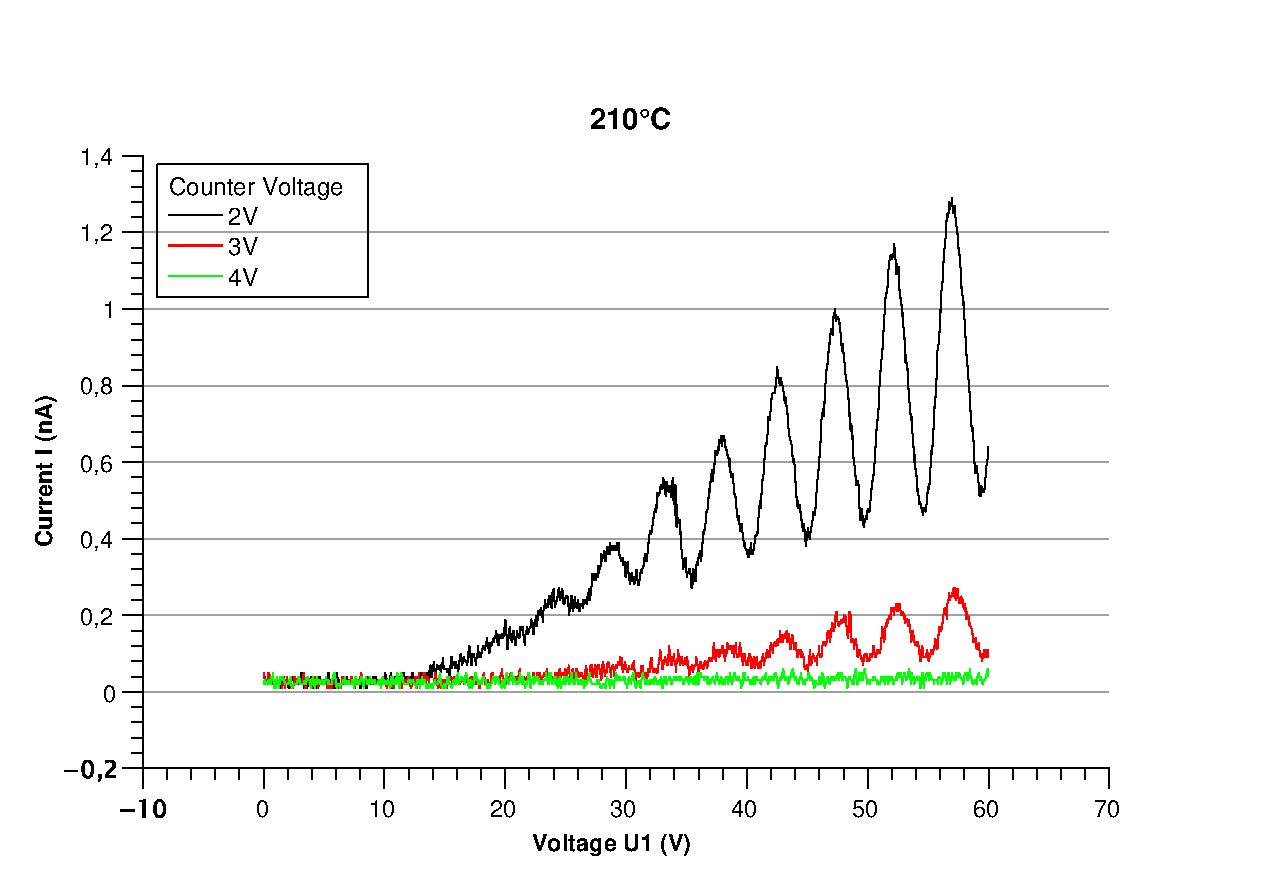
\includegraphics[width=8cm]{210.eps}
\caption{I(V) for 210°C}
\end{subfigure}
\end{center}
\end{figure}
\FloatBarrier

\begin{itemize}
    \item once \textit{ignition} of the tube occurs, the gas gets ionized and we can't record any meaningful data
    \item the extrema of the current are achieved for set values of the accelerating voltage and are independant of the applied counter voltage
    \item the separation between the peaks is independant of temperature and is about 5V
    \item the higher the counter voltage, the lower the current 
    \item the higher the counter voltage, the more minimum and maximum peaks are shifted to the right
    \item the higher the temperature, the lower the current
\end{itemize}

\noindent During the inelastic collision, the electron gives away its kinetic energy and excite and electron in the mercury atom. This excitation energy is represented on the graph as the peaks, where afterwards the current drops, because the electrons, that lost energy to the mercury atom, can't reach the anode anymore.
One can calculate the average distance of those peaks, and therefore find the excitation energy .
%we get the following result: one for 150,170,190,210 + average of all
In order to reduce the error on the excitation energy, one can take the several peaks and divide by the total amount of peaks. We obtain for the different temperatures: \[\begin{cases}
    \overline{E_{Hg,150^{\circ} C}} = 4.96 \text{eV} \\
    \overline{E_{Hg,170^{\circ} C}} = 5.00 \text{eV} \\
    \overline{E_{Hg,190^{\circ} C}} = 4.94 \text{eV} \\
    \overline{E_{Hg,210^{\circ} C}} = 4.79 \text{eV} 
\end{cases}\] This yields an average value of the excitation energy of Mercury of: \[ \boxed{\overline{E_{Hg}}=4.92 \ \text{eV}}\]

\noindent This information can be used to compute the wavelength of the emitted light during the transition between excited and ground state using Planck’s constant $h= 6.626 \cdot 10^{-34}$ Js and the speed of light $c = 3 \cdot 10^8$ ms$^{-1}$:
$$\Delta U = eU_1 = \frac{hc}{\lambda}$$
The resulting wavelength is: \[\boxed{\lambda = 252.0 \ \text{nm}}\]

%uncertainty
%mit theoretischen Wert vergleichen.

\subsubsection{Neon}
\begin{figure}[h]
    \centering
    \includegraphics[width = 14cm]{Neon.eps}
    \caption{I(V) of neon}
    \label{fig:my_label}
\end{figure}
\FloatBarrier

\noindent Repeating the same steps as for Mercury, we obtain: \[\boxed{\overline{E_{Ne}}=18.17 \ \text{eV}} \] and \[ \boxed{\lambda = 68.2 \ \text{nm}}\]

\section{Photoelectric effect}

\subsection{Setup}
\begin{wrapfigure}{r}{0.4 \textwidth}
\centering
    \includegraphics[width=0.3\textwidth]{kk_2.jpg}
    \caption{Photoelectric effect setup}
\end{wrapfigure}

We have at our disposal a gas discharge lamp filled with mercury, 6 different filters used as monochromators and 3 different apertures ranging from 2mm to 8mm that will reduce the lights intensity. The radiation of the gas lamp causes an emission of electrons from the cathode that are then accelerated to the positively charged anode and thus creates a current.

%graph modern physics with work function and stopping potential

\subsection{Method}

\subsubsection{Determination of Planck's constant}

The energy of an electron leaving the metal in the diode is given by: \[ hf = \frac{1}{2}m v^2 +\Phi_{cathode}\] where $\Phi_{cathode}$ is the work function of the metal. If a counter voltage is applied such that the current measured is 0, then the potential energy induced by the counter voltage is equal to the kinetic energy of the electrons (i.e. it negates it): \[ eV_0 = \frac{1}{2} m v^2\] Plugging this back in, we obtain a linear relationship, which enables us to determine Planck's constant:\begin{equation} V_0 = \frac{h}{e}f - \frac{\Phi_{cathode}}{e} \end{equation} Using the well-known relationship $f = \frac{c}{\lambda}$, one can determine the wavelength: $\lambda = \frac{c}{f}$. Using the set of filters we are provided, we can adjust the counter voltage in such a manner that the current becomes zero, at different wavelengths. When fitting the data with linear fits, the slope is then given by $slope = \frac{h}{e}$, from which Plancks constant can be determined: \[h= e \cdot slope \] The results are presented in the section below. 

\subsubsection{Characteristics of the photo diode}

In order to study the characteristics of the photo diode, one can record the current as a function of voltage and wavelength. This can be achieved by changing the voltage in steps of 2V from 0V to 30V for each filter and aperture setting, resulting in 15 curves. 

\subsection{Results}

\subsubsection{Determination of Planck's constant}

We record the values of the voltage, at which the current is 0, for each pair of wavelength and aperture setting.

\begin{center}
\begin{tabular}{c|c|ccc}
     \multicolumn{2}{c|}{ } & \multicolumn{3}{c}{Voltage (V)} \\
    \hline
    Frequency ($10^{14}$ Hz) & Wavelength (nm) & Aperture 8mm & Aperture 4mm & Aperture 2mm \\\hline
    5.196 & 577 & -0.668 & -0.663 & -0.651 \\
    5.491 & 546 & -0.801 & -0.789 & -0.772 \\
    6.876 & 436 & -1.375 & -1.371 & -1.327 \\
    7.402 & 405 & -1.580 & -1.579 & -1.526 \\
    8.214 & 365 & -1.849 & -1.860 & -1.841
\end{tabular}
\end{center}

\noindent With these values, we can create linear functions, which satisfy eq.(1) we get the stopping potential of each aperture: 

\[\begin{cases}
    V_0 = -3.945774 \cdot 10^{-15} + 1.394871 & \text{Aperture 2mm} \nonumber \\
    V_0 = -4.013946 \cdot 10^{-15} + 1.411107 & \text{Aperture 4mm} \nonumber \\
    V_0 = -3.957856 \cdot 10^{-15} + 1.371688 & \text{Aperture 8mm} \nonumber
\end{cases}\]

\noindent They are represented in the following graph:

\begin{figure}[ht]
    \centering
    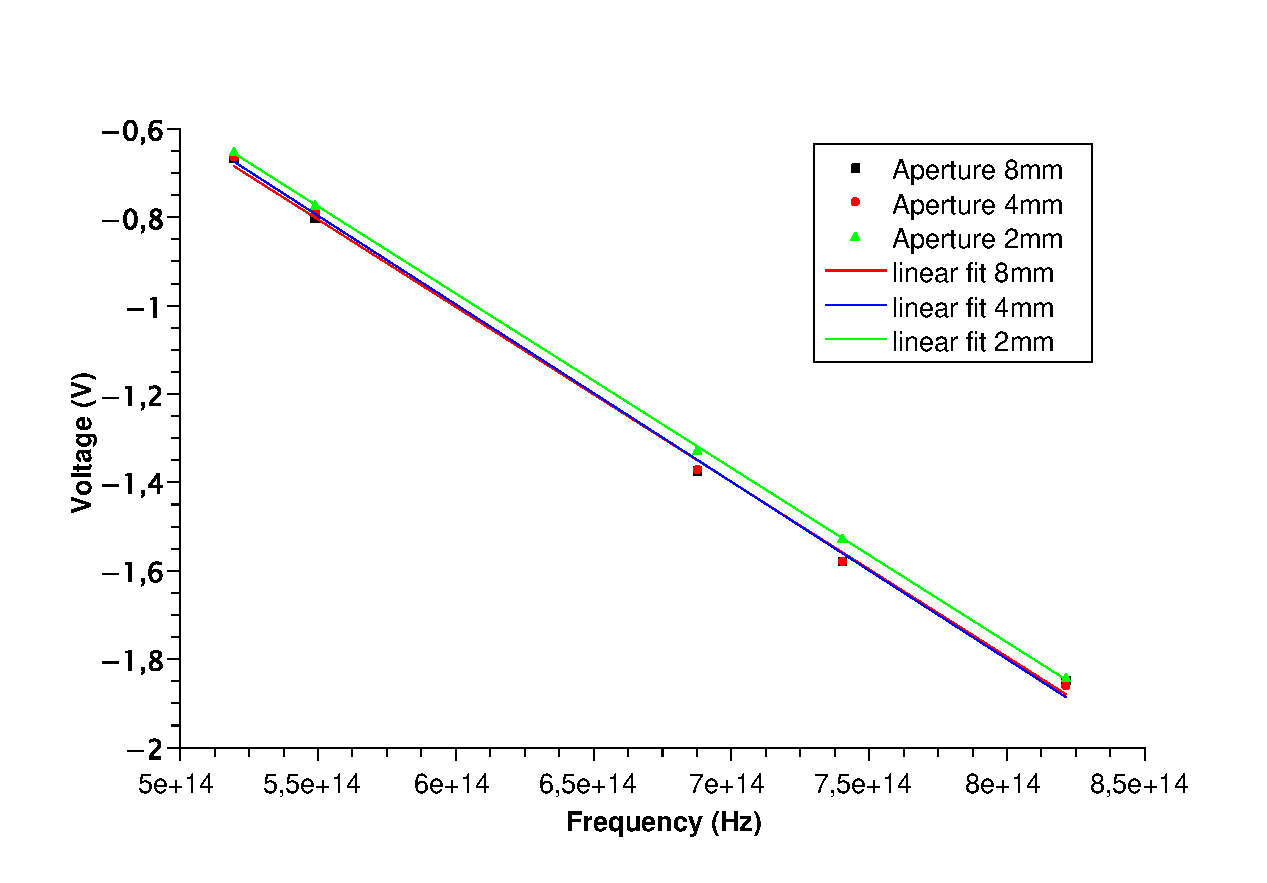
\includegraphics[width=14cm]{TP1_PhotoEffect_Part1_PlanckConst.eps}
    \caption{Voltage as a function of frequency}
    \label{fig:my_label}
\end{figure}
\FloatBarrier

\noindent Using as $e=-1.602\cdot 10^{-19}C$ the Planck constant for each fit is: \[\begin{cases}
    h_1 = 6.341 \cdot 10^{-34} \ \text{m}^2 \cdot \text{kg} \cdot \text{s}^{-1} \\
    h_2 = 6.431 \cdot 10^{-34} \ \text{m}^2 \cdot \text{kg}\cdot \text{s}^{-1} \\
    h_3 = 6.322 \cdot 10^{-34} \ \text{m}^2 \cdot \text{kg}\cdot \text{s}^{-1}
\end{cases}\]
Which in turn yields an average value of: $\bar{h} = 6.365 \cdot 10^{-34} \ \text{m}^2 \cdot \text{kg}\cdot \text{s}^{-1}$. The deviation to the theoretical value $h_{theo} = 6.626 \cdot 10^{-34} \ \text{m}^2 \cdot \text{kg}\cdot \text{s}^{-1}$ is $3.95\%$.

\subsubsection{Characteristics of the photo diode}
In order to study the characteristics of the photo diode, the current is recorded for variations in steps of 2V of the voltage. This is repeated at the same five wavelengths and each of the 3 aperture settings as before. Grouping the results for each aperture we get following curves:

\begin{figure}[ht]
\begin{subfigure}{0.3 \textwidth}
    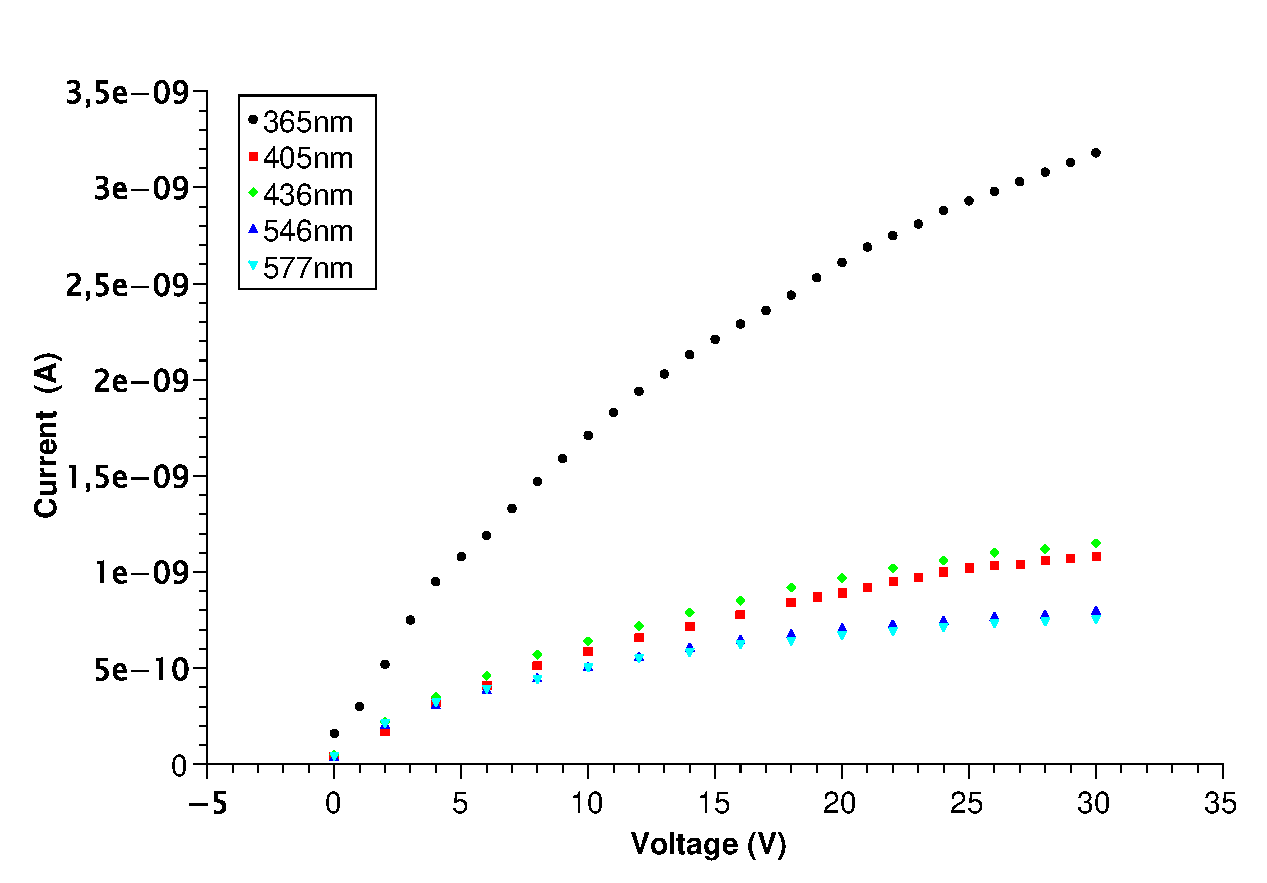
\includegraphics[width=5cm]{TP1_PhotoEffect_Part2_Aperture2mm.eps}
    \caption{Aperture 2mm}
\end{subfigure}
\begin{subfigure}{0.3 \textwidth}
    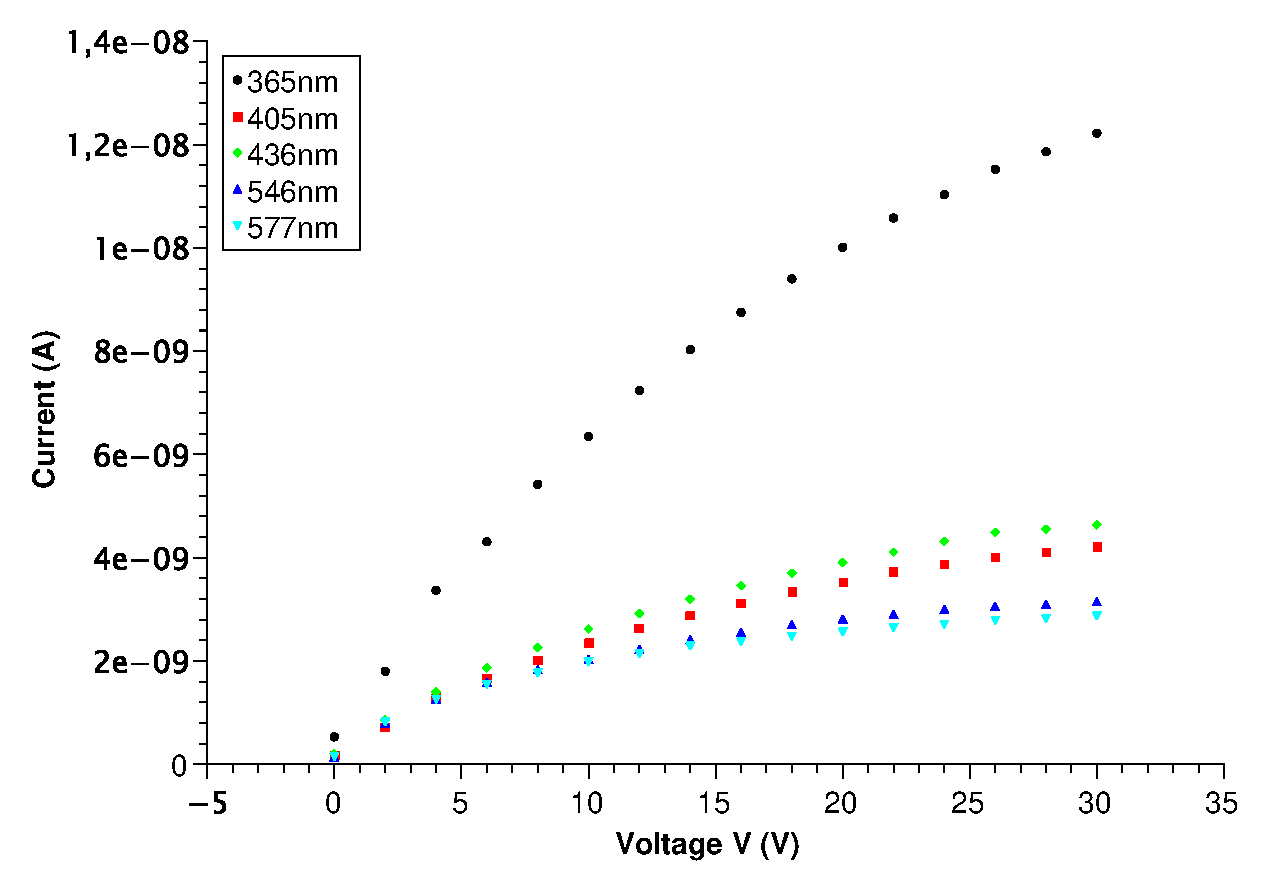
\includegraphics[width=5cm]{TP1_PhotoEffect_Part2_Aperture4mm.eps}
    \caption{Aperture 4mm}
\end{subfigure}
\begin{subfigure}{0.3 \textwidth}
    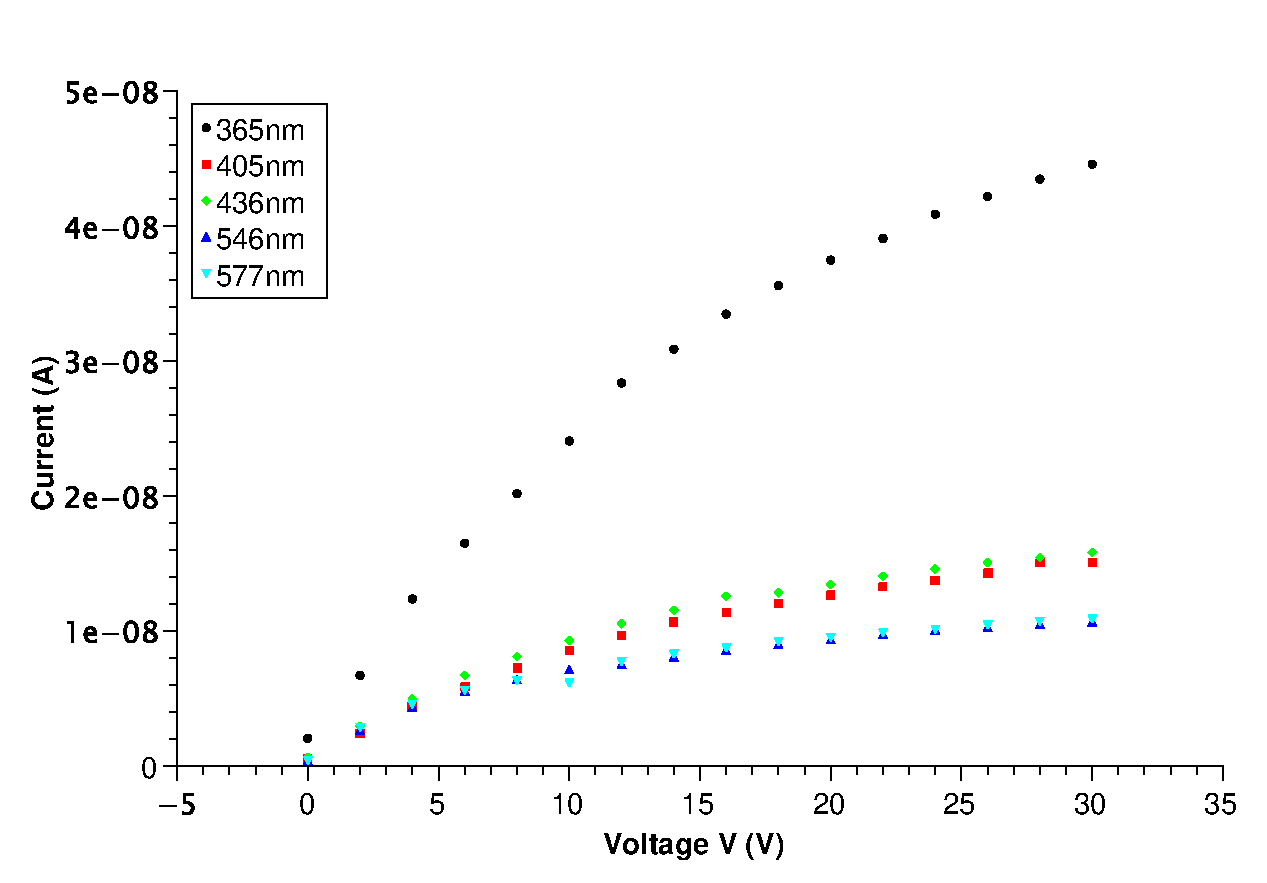
\includegraphics[width=5cm]{TP1_PhotoEffect_Part2_Aperture8mm.eps}
    \caption{Aperture 8mm}
\end{subfigure}
\end{figure}
\FloatBarrier 

\noindent For smaller wavelengths, i.e. higher energies of the photons, the current is higher for a given voltage. Generally, the current increases as the voltage increases, but the slope flattens gradually and seems to hit a plateau (especially for bigger wavelengths). The cutoff voltage is the same, regardless of aperture and wavelength. When comparing all three apertures, the trend arises, that with bigger aperture, the resulting current is higher.

\section{Conclusion}

The Franck-Hertz experiment was an effective way visually explain the quantization of energy levels inside atoms. On the other hand, with the photoelectric effect we could quantize and prove the existence of photons. In the first part of the TP, we were able to determine the excitation energy of both mercury and neon and their corresponding wavelength. We found an average excitation energy of mercury of $\overline{E_{Hg}}=4.92 \ \text{eV}$ with a wavelength of 252.0 nm. For neon we got $\overline{E_{Ne}}=18.17 \ \text{eV}$ with a wavelength of 68.2 nm. Then, for the second part, our task was to determine Planck's constant and experimentally found it to be $h = 6.365 \cdot 10^{-34} \ \text{m}^2 \cdot \text{kg}\cdot \text{s}^{-1}$. 

\section{Appendix}
\begin{proof}
Demonstartion for the validity of the following equation in the case of an elastic collision between electron and atom.

\begin{equation}
    \frac{\Delta E_e}{E^{initial}_e} = \frac{4m_e}{m_{gas}}
\end{equation}

As we are dealing with an elastic collision, conservation of energy
\begin{equation}
    \frac{1}{2}m_ev_e^2 = \frac{1}{2}m_ev_e^{'2}+\frac{1}{2}m_{Hg}v_{Hg}^2
\end{equation}

and conservation of momentum 

\begin{align}
    m_ev_e &= m_ev'_e + m_{Hg}v_{Hg} \nonumber\\
    v'_e &= \frac{m_{Hg}}{m_e}v_{Hg} - v_e 
\end{align}

If we now plug $v'_e$ into equation 3(conservation of energy) we get:
$$\frac{1}{2}m_ev_e^2 = \frac{1}{2}m_e(\frac{m_{Hg}}{m_e}v_{Hg} - v_e)^2+\frac{1}{2}m_{Hg}v_{Hg}^2$$

That can be simplified to:

$$\left(\frac{m_{Hg}^2}{m_e}+m_{Hg} \right)v_{Hg}^2 -2mg_{Hg}v_ev_{Hg} = 0$$
Solving for $v_{Hg}$:

$$v_{Hg} = \frac{2m_{Hg}v_e}{\frac{m_{Hg}^2}{m_e}+m_{Hg}}$$

Now we replace this expression into equation 4, we get:

$$v'_e = \frac{m_{Hg}}{m_e}\left(\frac{2m_{Hg}v_e} {\frac{m_{Hg}^2}{m_e}+m_{Hg}} \right) - v_e$$

We are interested in the change of energy of the electron which is equal to the change of kinetic energy of the mercury atom:
\begin{align}
    \Delta E_e &=  \frac{1}{2}m_{Hg}^2 \nonumber \\
    &= \frac{1}{2}m_e v_e ^2-\frac{1}{2}m_e v_e'^2 \nonumber
\end{align}

With $$E_e^{initial} = \frac{1}{2}m_ev-e^2$$ we can simplify the previous expression:

\[\Delta E_e = E_e^{initial} \left(1-\frac{1}{2}m_e \left(\frac{m_{Hg}-m_e}{m_{Hg}+m_e}\right)^2 v_e^2 \right)\]
\[\frac{\Delta E_e}{E_e^{initial}} = \frac{4m_{Hg}m_e}{\left(m_{Hg}+m_e \right)^2}\nonumber \]

As $m_{Hg} \gg m_e$ we can conclude that


\[\frac{\Delta E_e}{E_e^{initial}} = \frac{4m_e}{m_{Hg}}\]
\end{proof}

Plugging in the values we finally obtain:

\[ \left( \frac{\Delta E_e}{E_e^{initial}} \right)_{Hg} \simeq 3.1 \cdot 10^{-4}\]
\[ \left( \frac{\Delta E_e}{E_e^{initial}} \right)_{Ne} \simeq 3.0 \cdot 10^{-3}\]

This implies the energy losses due to elastic collisions are negligible.

\printbibliography

\end{document}
